\documentclass{beamer}

\usetheme{MagdeburgFIN}
\usefonttheme{structurebold}
\usepackage{graphicx}
\usepackage{float}
\usepackage{url}
\usepackage{pdfpages}

\title{Semi Supervised Support Vector Machines}
\author{Bethe, Herdick}
\date{6.12.2016}
\institute{Classification Algorithms FIN OvGU}

\begin{document}

% avoid "figure:" in image captions
\setbeamertemplate{caption}{\raggedright\insertcaption\par}

% easy properly scaled full-size images
\newcommand {\framedgraphic}[2] {
    \begin{frame}{#1}
        \begin{center}
            \includegraphics[width=\textwidth,height=0.8\textheight,keepaspectratio]{#2}
        \end{center}
    \end{frame}
}

\begin{frame}[plain]
\titlepage
\end{frame}


\section[Agenda]{}
\begin{frame}
\frametitle{Agenda}
\tableofcontents
\end{frame}

\section{Idee der S3VMs}
\begin{frame}
\frametitle{Idee der S3VMs}
    \begin{itemize}
        \item Gelabelte Daten sind teuer
        \item Also: Ungelabelte Daten zus\"atzlich verwenden
        \item Wie kann man die ungelabelten Daten dem Optimierungsterm der SVMs hinzuf\"ugen?
        \item Wie findet man die neue Hyperebene?
    \end{itemize}
\end{frame}




\section{Erinnerung: SVMs}

\begin{frame}
\frametitle{Optimierungsproblem der Soft-Margin SVM}
    \begin{itemize}
    	\item Alte Formulierung:
    	\begin{itemize}
    		\item $min_{h,b,\chi} \sum_{i=1}^l \xi_i + \lambda \|h\|^2_{H_k}$
    		\item $y_i(h(x_i) + b) \geq 1 - \xi_i, \forall i=1,...,l$
    		\item $\xi_i \geq 0$
    	\end{itemize}
    	\item Optimierungsproblem: $min_h \sum_{i=1}^l (1-y_i f(x_i))_+ + \lambda \|h\|^2_{H_k}$
    	\item Klassifikation: $f(x) = sgn\left(\sum_{i=1}^{SV} \alpha_i y_i k(x, x_i)\right)$
    \end{itemize} 
\end{frame}


\section{Optimierungsproblem der S3VM}

\begin{frame}
\frametitle{Optimierungsproblem der S3VM}
    $min_h \sum_{i=1}^l (1-y_i f(x_i))_+ + \lambda \|h\|^2_{H_k} + \lambda_2 \sum_{i=l+1}^n (1- |f(x_i)|)_+$
\end{frame}



\section{Loss-Funktionen}

\begin{frame}
    \frametitle{Hinge-Loss-Funktion} 
    \begin{tabular}{cl}  
        \begin{tabular}{c}                                       
        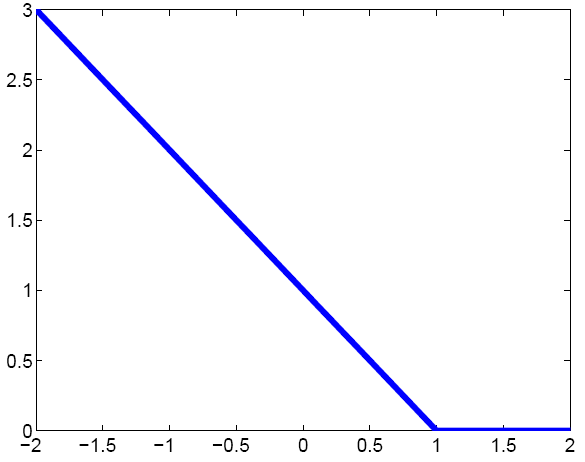
\includegraphics[scale=0.2]{img/hinge_loss_function.png} 
    \end{tabular}
    & \begin{tabular}{l}
    \parbox{0.5\linewidth}{
        \begin{itemize}
            \item Bewerten die Klassifikation eines Punktes
            \item $\mathcal{L}(y, f(x)) = max(0, 1 - y f(x))$
        \end{itemize}
    }
    \end{tabular}  \\
    \end{tabular}
\end{frame}

\begin{frame}
    \frametitle{Hat-Loss-Funktion} 
    \begin{tabular}{cl}  
        \begin{tabular}{c}                                       
        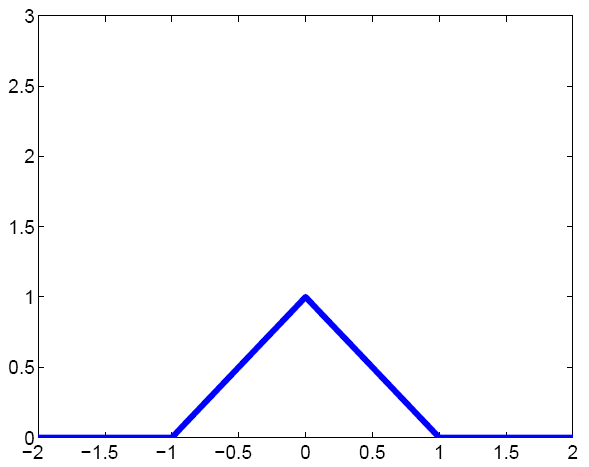
\includegraphics[scale=0.2]{img/hat_loss_function.png} 
    	\end{tabular}
    & \begin{tabular}{l}
    \parbox{0.5\linewidth}{
        \begin{itemize}
        \item Ungelabelte Daten haben keine bevorzugte Seite der Hyperebene
        \item Den ungelabelten Daten wird $y_i = sign(f(x))$ zugewiesen. 
        \item Da $sign(f(x))*f(x) = |f(x)|$, gilt f\"ur die ungelabelten Daten $\mathcal{L}(f(x)) = max(0, 1-|f(x)|)$
        \end{itemize}
    }
    \end{tabular}  \\
    \end{tabular}
\end{frame}

\begin{frame}
    \frametitle{Surrogate-Funktionen}
    
    \begin{itemize}
    	\item Loss-Funktionen nicht differenzierbar
    	\item Ersetze durch \"ahnliche "Surrogates"
    \end{itemize}
    \begin{columns}[onlytextwidth]
        \begin{column}{.45\textwidth}
            \begin{figure}
                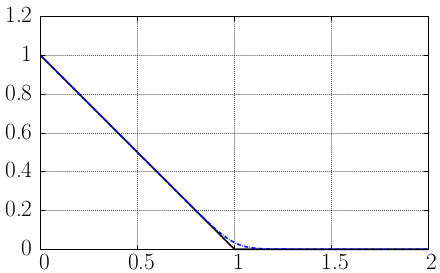
\includegraphics[width=\textwidth]{img/hinge_loss_surrogate_function.png}
                \caption{$\mathcal{L}_{HINGE}(y, f(x)) = \frac{1}{\gamma} log(1 + exp(\gamma(1-y_i' f(x_i))))$}
            \end{figure}
        \end{column}
        \hfill
        \begin{column}{.45\textwidth}
            \begin{figure}
                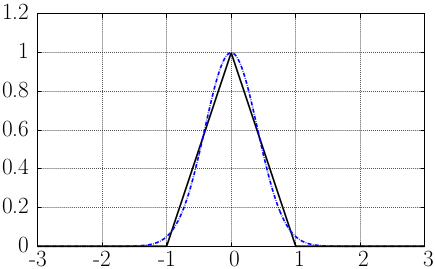
\includegraphics[width=\textwidth]{img/hat_loss_surrogate_function.png}
                \caption{$\mathcal{L}_{HAT}(f(x)) = exp(-3(f(x_{l+i}))^2)$}
            \end{figure}
        \end{column}
    \end{columns}
\end{frame}




\section{L\"osung des Optimierungsproblems}

\begin{frame}
	\frametitle{L\"osung des Optimierungsproblems}
	\textbf{Kontinuierlich}
	\begin{itemize}
		\item Problem 1: Optimierungsfunktion ist nicht konvex $\rightarrow$ numerisches Verfahren n\"otig
		\item Idee: Simulated Annealing
		\begin{itemize}
			\item Fixiere Labeling und erh\"ohe Einfluss $\lambda_2$ iterativ
			\item Initiall\"osung ganz ohne ungelabelte Daten
			\item Berechne Ebene und Labeling jede Iteration neu
		\end{itemize}
	\end{itemize}
\end{frame}

\begin{frame}
    \frametitle{L\"osung des Optimierungsproblems}
    \begin{itemize}
        \item Quasi-Newton Ann\"aherung
        \begin{itemize}
            \item Loss-Funktionen m\"ussen durch kontinuierliche "Surrogates" ersetzt werden
            \item Problem der nicht konvexen Hat-Loss-Funktion durch mithilfe des Quasi-Newtonschen Verfahrens umgehen
            \item \"Uber verschiedene Optimierungsverfahren kann der Aufwand dieser Methode gedr\"uckt werden
        \end{itemize}
    \end{itemize}
\end{frame}

\begin{frame}
    \frametitle{L\"osung des Optimierungsproblems}
    \textbf{Kombinatorisch}
    \begin{itemize}
    	\item Lokale Optima bei kontinuierlicher Optimierung m\"oglich
        \item Idee: Teste jede m\"ogliche Labelzuweisung f\"ur fixe Hyperebene
        \item Branch and bound: Aufspannen des Suchbaums
        \begin{itemize}
        	\item Depth-first search
        	\item "Prunen" von Teilb\"aumen mit schlechterem Labeling
        \end{itemize}
        \item Findet globales Optimum, aber Worst Case von $O(2^n)$
    \end{itemize}
\end{frame}


\section{Ergebnisvergleich}

\begin{frame}
	\frametitle{Ergebnisvergleich}
	\begin{figure}
	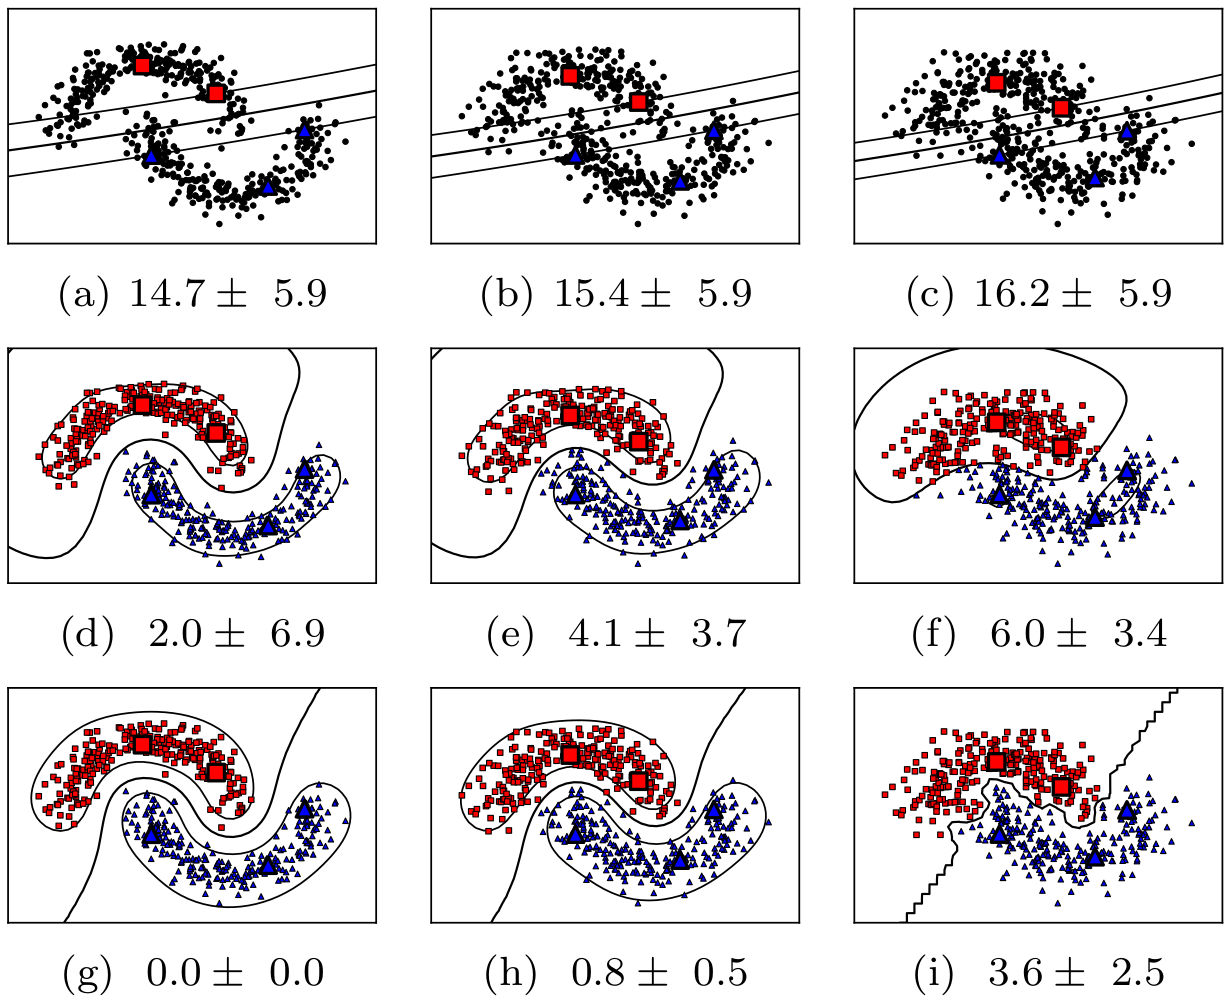
\includegraphics[width=\linewidth,height=.7\textheight,keepaspectratio]{img/example_results.png}
    \caption{$LIBSVM$, $UniverSVM$ und $QN-S^3VM$}
	
	\end{figure}
\end{frame}


\section{Quellen}

\begin{frame}
\frametitle{Quellen}
\begin{itemize}
\item Gieseke, F., Airola, A. Pahikkala, T., Kramer, O. (2012). Sparse Quasi-Newton optimization for semi-supervised support vector machines
\item N\"urnberger, A. (2016). Advanced Topics in Machine Learning: Semi-Supervised Learning
\end{itemize}
\end{frame}


\begin{frame}
\frametitle{Danke f\"ur eure Aufmerksamkeit!}
\end{frame}


\end{document}
